% Adapted from https://github.com/theflyingwolves/NUS-Slides-Latex-Template
% Original template copyright 2016 Wang Kunzhen, GPL v2 with template-use permission.
\documentclass[xcolor=dvipsnames,aspectratio=43]{beamer}

\usetheme{Malmoe}
\usepackage{booktabs}
\usepackage{graphicx}
\usepackage{tabularx}
\usepackage{array}
\usepackage{ragged2e}
\usepackage{amsmath}

\definecolor{nus-orange}{RGB}{239,124,0}
\definecolor{nus-white}{RGB}{255,255,255}
\definecolor{nus-blue}{RGB}{0,61,124}
\definecolor{nus-black}{RGB}{0,0,0}
\definecolor{soft-blue}{RGB}{232,240,248}
\definecolor{soft-orange}{RGB}{253,239,222}

\setbeamercolor{section in head/foot}{bg=nus-blue,fg=nus-white}
\setbeamercolor{subsection in head/foot}{bg=nus-blue,fg=nus-white}
\setbeamercolor{frametitle}{bg=nus-orange,fg=nus-black}
\setbeamercolor{title}{bg=nus-orange,fg=nus-white}
\setbeamercolor{alerted text}{fg=nus-orange}
\setbeamercolor{block title}{fg=nus-white,bg=nus-blue}
\setbeamercolor{block body}{fg=nus-black,bg=soft-blue}
\setbeamercolor{exampleblock title}{fg=nus-black,bg=nus-orange}
\setbeamercolor{exampleblock body}{fg=nus-black,bg=soft-orange}
\setbeamertemplate{title page}[default][colsep=-4bp,rounded=true,shadow=true]
\setbeamertemplate{navigation symbols}{}
\setbeamertemplate{footline}[frame number]
\setbeamersize{text margin left=0.55cm,text margin right=0.55cm}

\newcommand{\source}[1]{%
  \vfill\par\begingroup\raggedright\tiny\color{gray}Source: #1\par\endgroup
}
\newcommand{\metric}[2]{\textcolor{nus-blue}{\textbf{#1}}\\[-1mm]{\small #2}}

\title{Predicting Singapore HDB Monthly Rent}
\subtitle{CS5228 Project Progress Report -- Group 44}
\author[Group 44]{%
  \texorpdfstring{%
    \begin{tabular}{@{}l@{\hspace{1.0cm}}l@{}}
      Han Linxuan    & A0350911M \\
      Sun Shenghe    & A0354849L \\
      Zhang Yuhong   & A0356795H \\
      Zhang Zhexuan  & A0355290A
    \end{tabular}%
  }{Han Linxuan A0350911M; Sun Shenghe A0354849L; Zhang Yuhong A0356795H; Zhang Zhexuan A0355290A}%
}
\institute[National University of Singapore]{
  School of Computing\\
  National University of Singapore
}
\titlegraphic{
\includegraphics[width=1.75cm]{assets/nus-logo}}
\date{September 2026}

\begin{document}

\begin{frame}
  \titlepage
\end{frame}

\begin{frame}{Problem and project goals}
\begin{columns}[T,totalwidth=\textwidth]
  \begin{column}{0.58\textwidth}
    \begin{block}{Prediction task}
      Estimate the monthly rent of an HDB flat from its approval month,
      location, flat characteristics and permitted auxiliary data.
    \end{block}
    \vspace{0.15cm}
    \begin{itemize}
      \item Metric: root mean squared error (RMSE)
      \item Output: one rent prediction for each of 50,000 test rows
      \item Main challenge: future rents must be predicted from historical transactions
    \end{itemize}
  \end{column}
  \begin{column}{0.38\textwidth}
    \begin{exampleblock}{Core research question}
      Can historical comparable rents improve future HDB rental forecasts as
      market conditions change?
    \end{exampleblock}
    \vspace{0.15cm}
    \scriptsize We also examine location effects, temporal stability and the
    sources of large prediction errors.
  \end{column}
\end{columns}
\source{CS5228 project page and Kaggle competition description}
\end{frame}

\begin{frame}{Data and prediction horizon}
\small
\begin{columns}[T,totalwidth=\textwidth]
  \begin{column}{0.48\textwidth}
    \begin{block}{Core data}
      \begin{itemize}
        \item 150,000 labelled rows
        \item Jan 2021 to Mar 2025
        \item 50,000 test rows
        \item Mar 2025 to Jul 2026
        \item Target range: SGD 300 to 7,600
      \end{itemize}
    \end{block}
  \end{column}
  \begin{column}{0.48\textwidth}
    \begin{block}{Auxiliary data}
      \begin{itemize}
        \item HDB block coordinates and attributes
        \item MRT stations, malls and primary schools
        \item COE and stock-price indicators (tested, not retained)
      \end{itemize}
    \end{block}
    \begin{alertblock}{Consequence}
      The test dates cover a 17-month span ending in Jul 2026.
      Time extrapolation matters as much as model fit.
    \end{alertblock}
  \end{column}
\end{columns}
\source{Official course dataset; local data audit}
\end{frame}

\begin{frame}{Rental levels changed substantially over time}
  \centering
  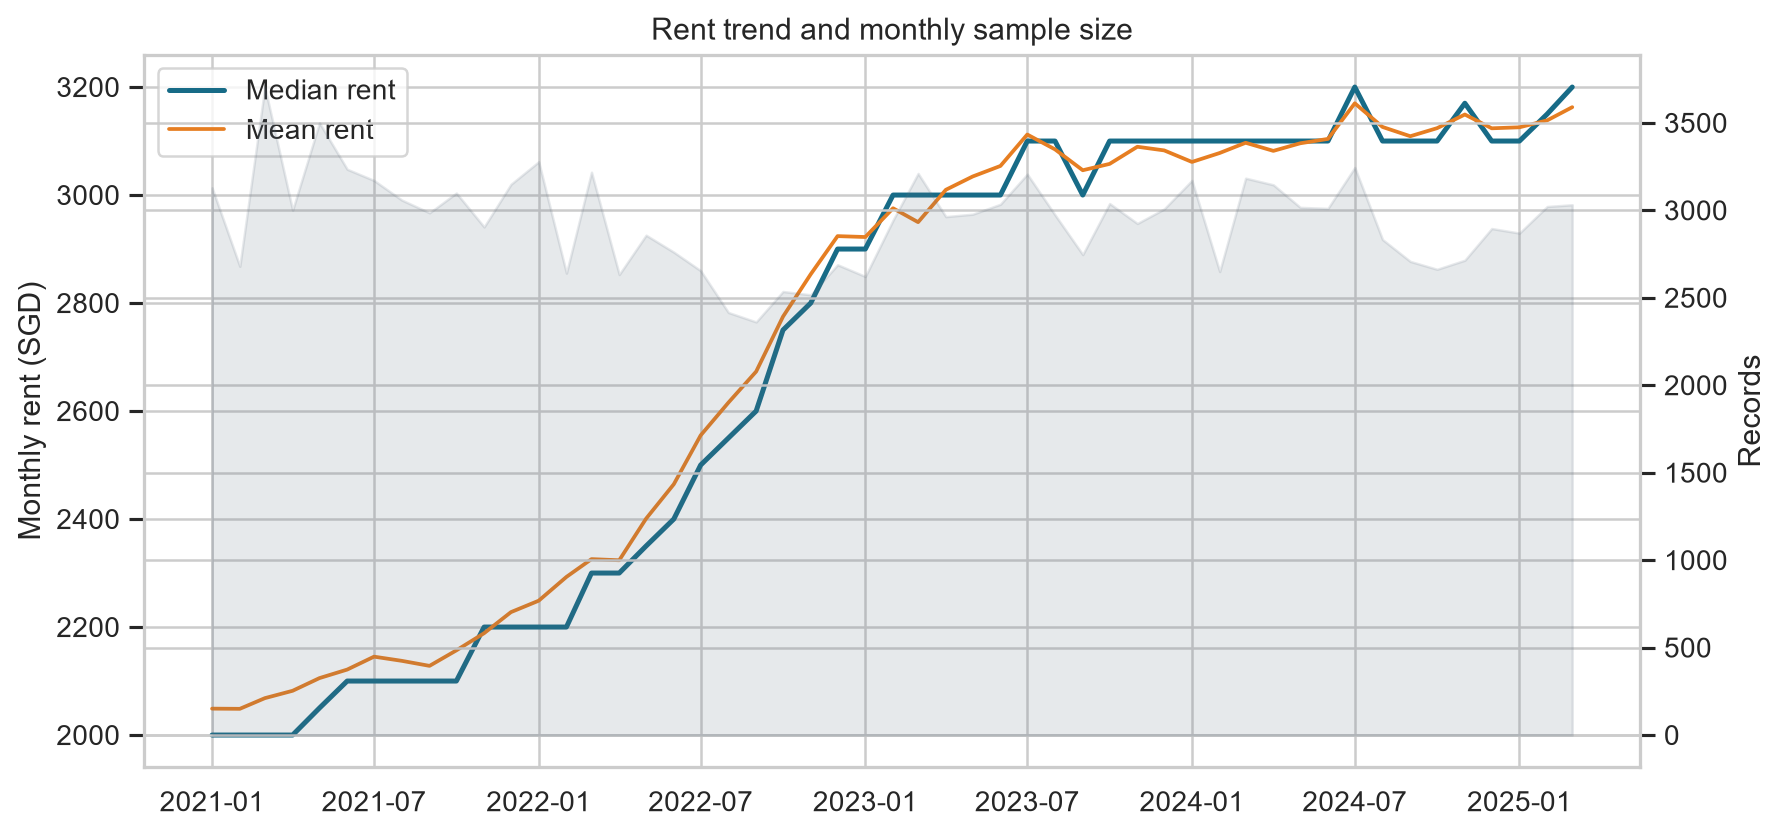
\includegraphics[width=0.94\textwidth,height=0.69\textheight,keepaspectratio]{assets/eda_monthly_trend.png}
  \vspace{-1mm}

  \small Median rent rose from about SGD 2,000 in early 2021 to around SGD 3,200 by early 2025.
  A random split would mix different market regimes and overstate future performance.
\source{Reproducible EDA on the 150,000 training rows}
\end{frame}

\begin{frame}{Rent varies across locations and contains difficult tails}
\begin{columns}[T,totalwidth=\textwidth]
  \begin{column}{0.58\textwidth}
    \centering
    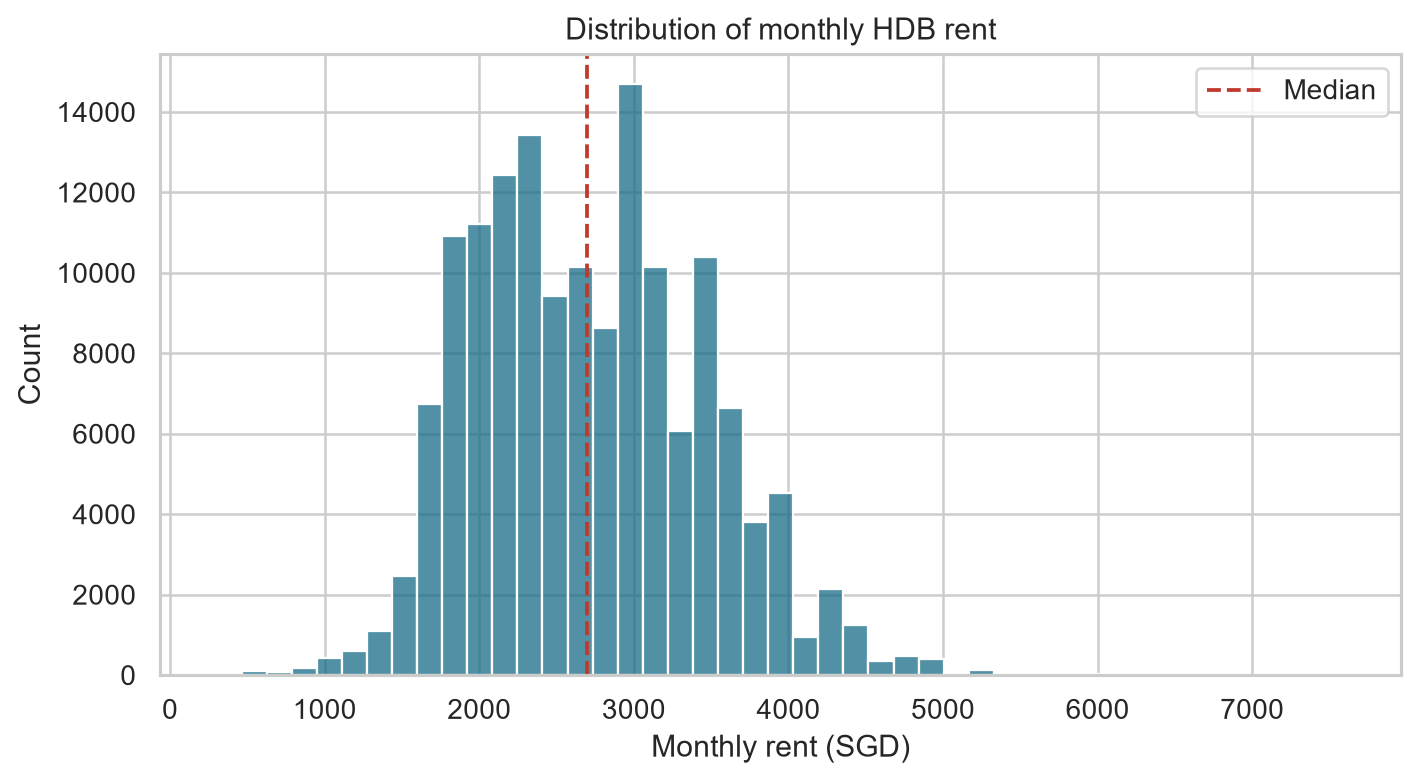
\includegraphics[width=\textwidth,height=0.57\textheight,keepaspectratio]{assets/eda_target_distribution.png}
    \small Overall median: SGD 2,700
  \end{column}
  \begin{column}{0.38\textwidth}
    \footnotesize
    \begin{block}{Town medians}
    \begin{tabular}{@{}lr@{}}
      \toprule
      Town & SGD \\
      \midrule
      Central & 3,000 \\
      Bukit Timah & 3,000 \\
      Bukit Merah & 2,900 \\
      Ang Mo Kio & 2,500 \\
      Bedok & 2,500 \\
      Woodlands & 2,500 \\
      \bottomrule
    \end{tabular}
    \end{block}
    Town medians differ, but this comparison also reflects date and flat-mix differences.
  \end{column}
\end{columns}
\vspace{1mm}
\small The distribution is multi-modal and includes unusually low rents, so we also analyse errors by rent band.
\source{Reproducible EDA summaries on the 150,000 training rows}
\end{frame}

\begin{frame}{Preprocessing and feature design}
\small
\begin{columns}[T,totalwidth=\textwidth]
  \begin{column}{0.47\textwidth}
    \begin{block}{Data preparation}
      \begin{itemize}
        \item Canonicalise text and flat-type formats
        \item Remove constant inputs: furnished and fee
        \item Audit 425 exact duplicate rows without automatic deletion
        \item Preserve raw files; validate schemas, hashes and output IDs
      \end{itemize}
    \end{block}
  \end{column}
  \begin{column}{0.51\textwidth}
    \begin{block}{Feature groups}
      \begin{itemize}
        \item Time, flat size, model and lease age
        \item Block, town, planning area and region
        \item Distance and counts for MRT, malls and schools
        \item Past-only comparable rents and local market momentum
      \end{itemize}
    \end{block}
  \end{column}
\end{columns}
\begin{alertblock}{Leakage control}
  Historical rent features use only months strictly earlier than each predicted row.
\end{alertblock}
\source{Project feature pipeline and automated data-contract tests}
\end{frame}

\begin{frame}{Chronological evaluation design}
\small
\begin{columns}[T,totalwidth=\textwidth]
  \begin{column}{0.56\textwidth}
    \begin{block}{Primary comparison}
      Expanding training data followed by future validation windows.
      The latest split trains on 141,076 rows through Dec 2024 and validates
      on 8,924 rows from Jan--Mar 2025.
    \end{block}
    \begin{itemize}
      \item Matched rows and preprocessing within each comparison
      \item Later screens fix seeds and 1,600-tree budgets
      \item Rolling three-month folds plus older-year and sixteen-month stress windows
      \item RMSE for selection; MAE and signed bias for diagnosis
    \end{itemize}
  \end{column}
  \begin{column}{0.41\textwidth}
    \begin{exampleblock}{Why this matters}
      The public leaderboard covers about half of the hidden test set.
      Local stability reduces dependence on one public split.
    \end{exampleblock}
    \vspace{0.1cm}
    \begin{alertblock}{Interpretation}
      Historical features never use validation labels. Overlapping stress
      windows test robustness but are not independent test sets.
    \end{alertblock}
  \end{column}
\end{columns}
\source{Project validation code and Kaggle evaluation description}
\end{frame}

\begin{frame}{CatBoost leads the initial model screen}
  \centering
  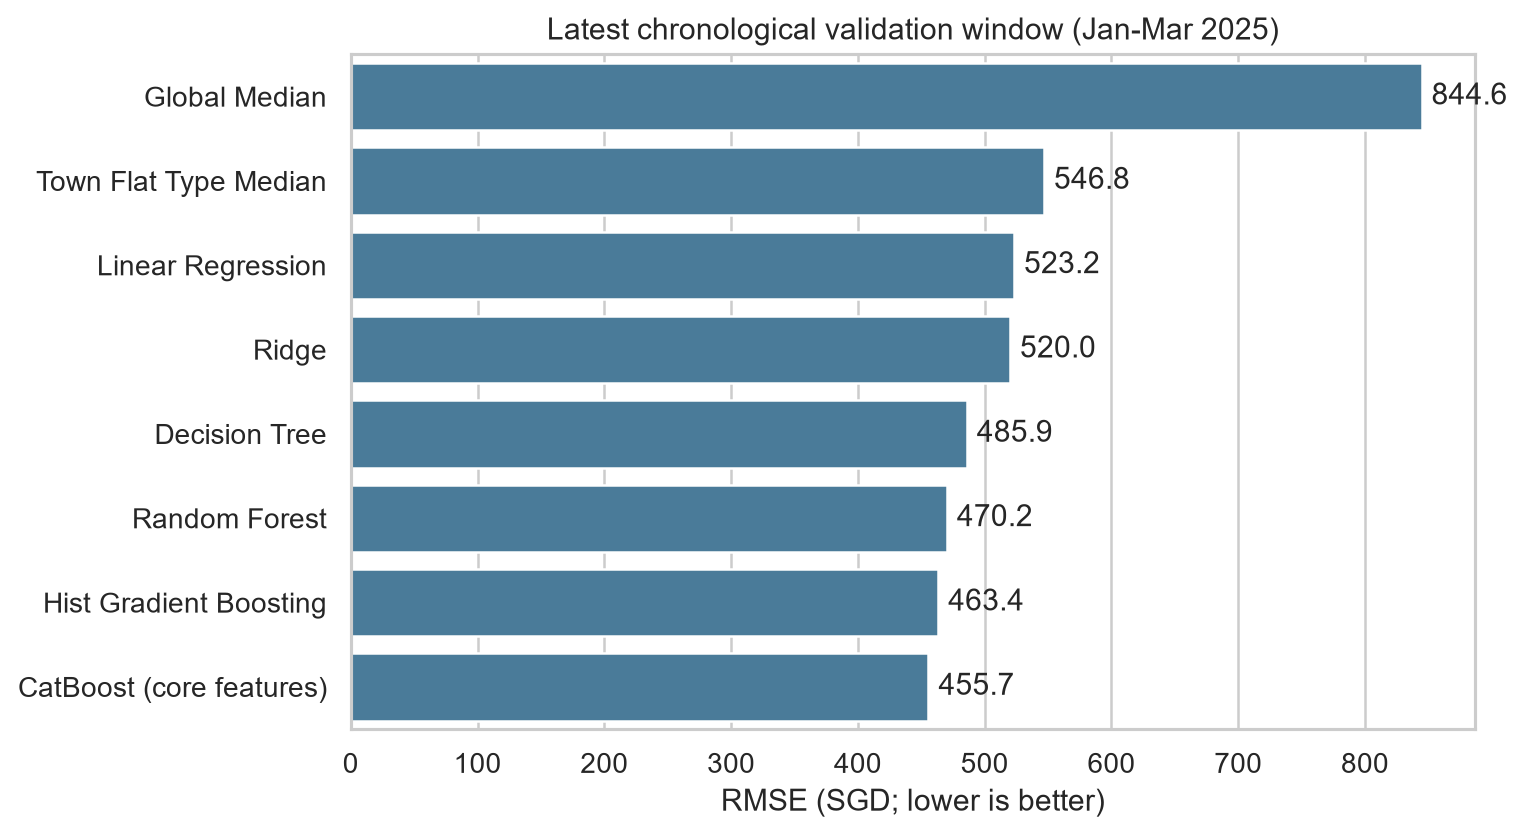
\includegraphics[width=0.93\textwidth,height=0.70\textheight,keepaspectratio]{assets/latest_model_comparison.png}
  \vspace{-1mm}

  \small All trained models use the same core inputs and rows; the two median rules use raw group summaries. CatBoost uses validation-based early stopping here, so this is an initial screen rather than a fixed-budget family benchmark.
\source{Jan-Mar 2025 validation; Prokhorenkova et al., NeurIPS 2018 for CatBoost}
\end{frame}

\begin{frame}{Staged model and feature changes reduced RMSE}
\begin{columns}[T,totalwidth=\textwidth]
  \begin{column}{0.52\textwidth}
    \centering
    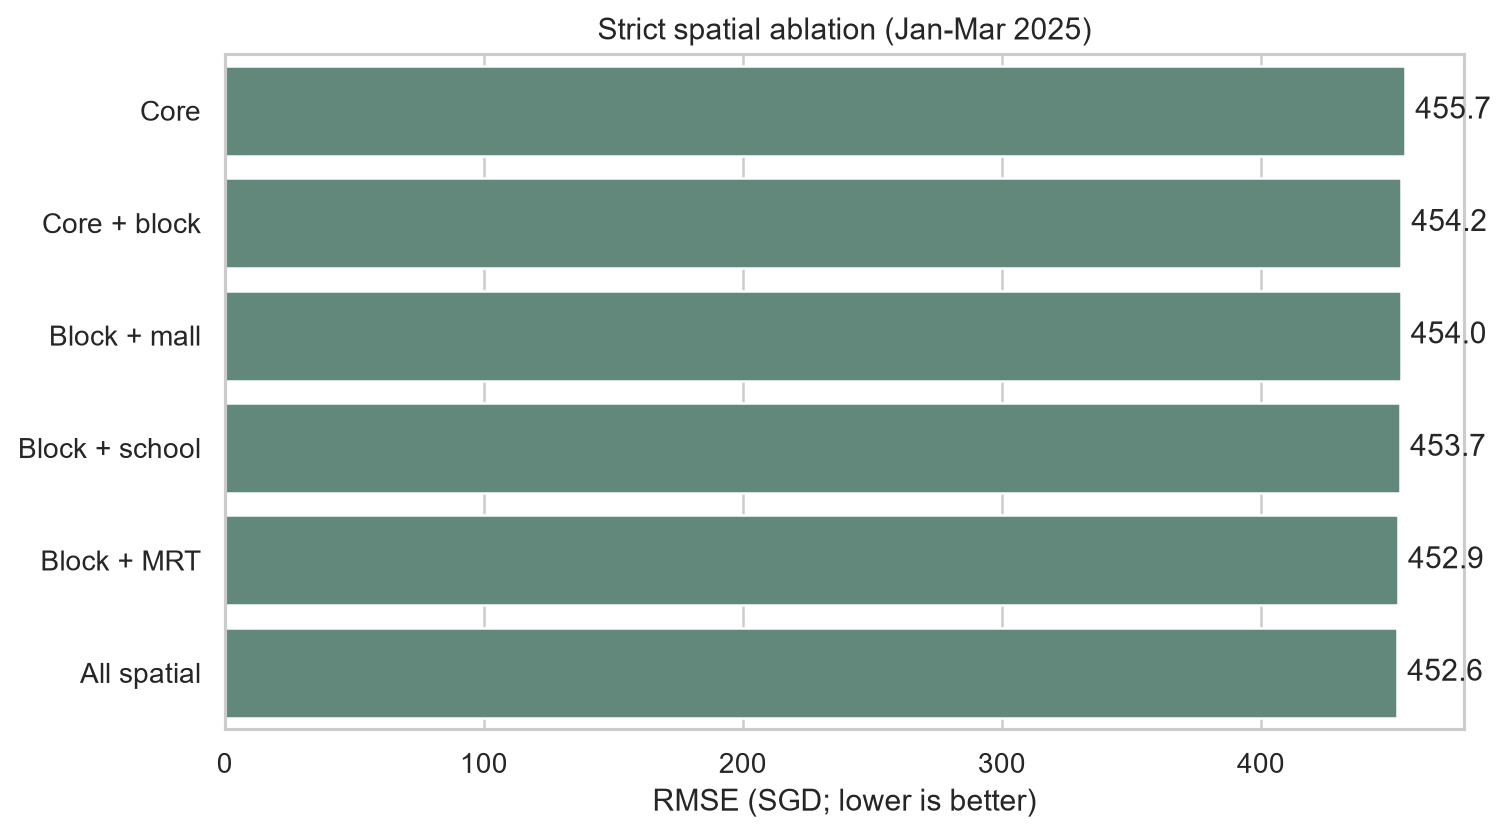
\includegraphics[width=\textwidth,height=0.56\textheight,keepaspectratio]{assets/spatial_ablation.png}
  \end{column}
  \begin{column}{0.44\textwidth}
    \small
    \resizebox{\linewidth}{!}{%
    \begin{tabular}{@{}lr@{}}
      \toprule
      Candidate & RMSE \\
      \midrule
      CatBoost core & 455.71 \\
      Spatial + past rent & 450.04 \\
      Adaptive market ensemble & 445.52 \\
      History diversity & 440.89 \\
      Local trend ensemble & 440.76 \\
      Recent-window stacking & \textbf{440.66} \\
      \bottomrule
    \end{tabular}}
    \vspace{0.25cm}

    The left chart isolates spatial additions. The table records successive pipeline versions, so its gains combine feature, target and ensemble changes.
  \end{column}
\end{columns}
\source{Jan-Mar 2025 validation; later candidates use two seeds and 1,600 trees per component}
\end{frame}

\begin{frame}{Current ensemble design}
\small
\begin{columns}[T,totalwidth=\textwidth]
  \begin{column}{0.48\textwidth}
    \begin{block}{Normal-history view}
      CatBoost predicts rent directly and as a residual from a past-only market estimate.
      Local town-flat-type momentum features describe recent changes.
    \end{block}
  \end{column}
  \begin{column}{0.48\textwidth}
    \begin{block}{Stale-history view}
      Eligible training rows receive a second feature view that hides the latest
      six months of history. The original and augmented copies split that row's weight.
    \end{block}
  \end{column}
\end{columns}
\vspace{0.25cm}
\begin{exampleblock}{Eight components}
  Two history views $\times$ two targets $\times$ two random seeds.
  The mainline averages all components equally. Residual models add the past-only
  market estimate back at prediction time. Every component uses all permitted history at inference.
\end{exampleblock}
Each component uses 1,600 trees, depth 8, learning rate 0.04 and L2 regularisation 6.
CatBoost was retained after bounded XGBoost tests and predefined blends failed to improve the same validation windows.
\source{Current configuration, model metadata and frozen stacking study}
\end{frame}

\begin{frame}{Current mainline still struggles at rent extremes}
\begin{columns}[T,totalwidth=\textwidth]
  \begin{column}{0.59\textwidth}
    \centering
    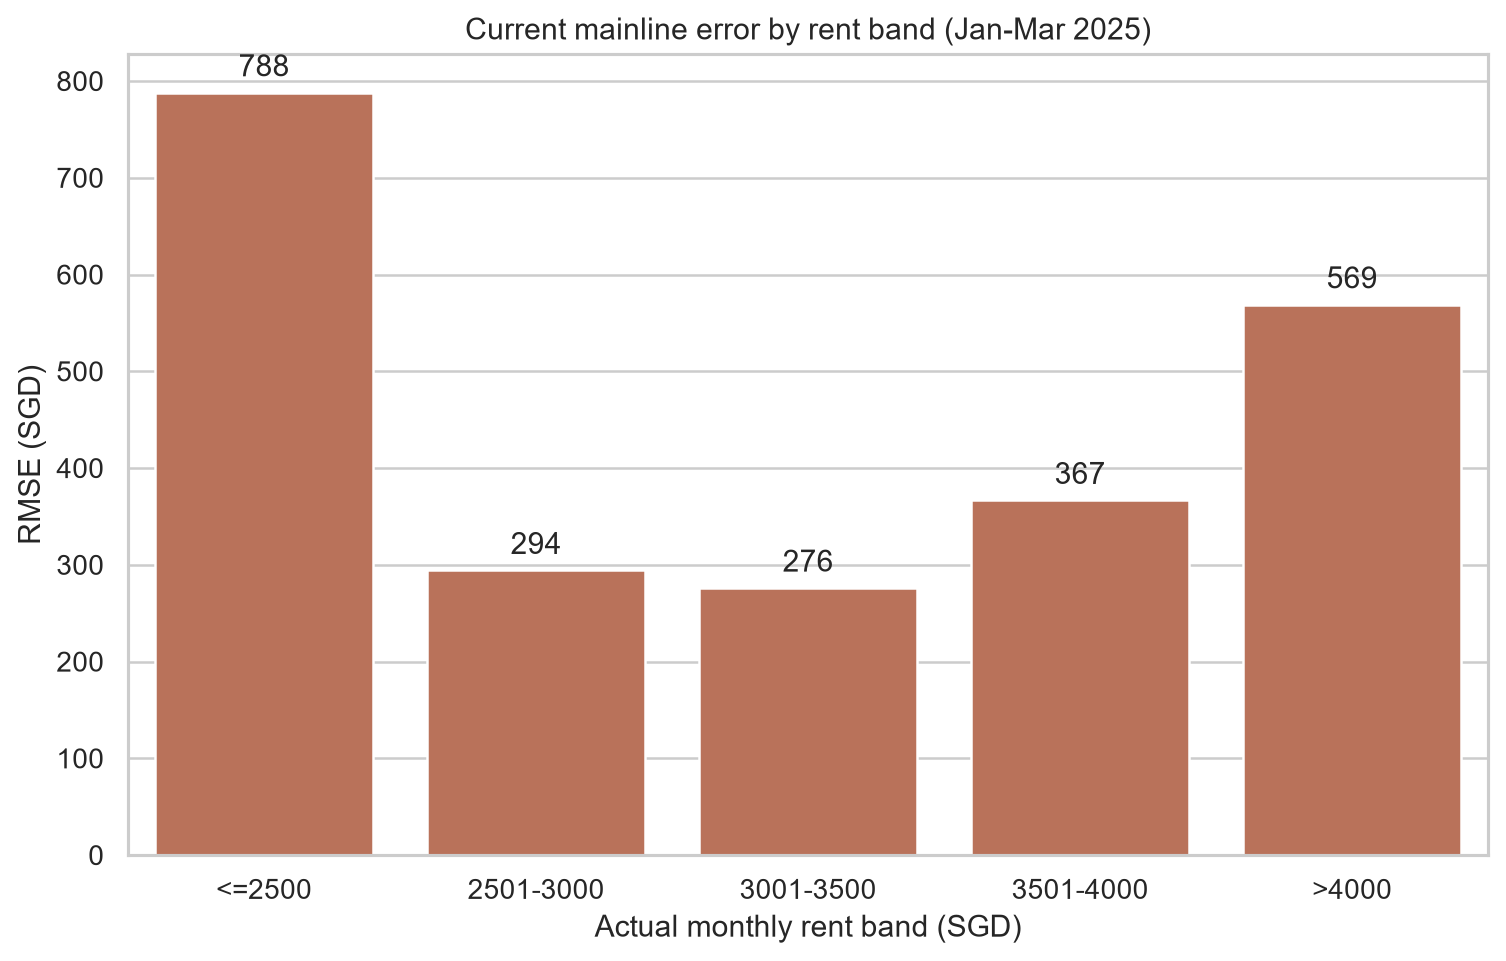
\includegraphics[width=\textwidth,height=0.55\textheight,keepaspectratio]{assets/error_by_rent_band.png}
  \end{column}
  \begin{column}{0.39\textwidth}
    \footnotesize
    \begin{itemize}
      \item The chart uses the selected 440.76-RMSE mainline on all 8,924 validation rows.
      \item At or below SGD 2,500, RMSE is 788 with positive bias; this band mixes ordinary low rents and suspected anomalies.
      \item Rents above SGD 4,000 also remain difficult.
      \item Jan 2025 RMSE is 456, versus 431 in Mar 2025.
    \end{itemize}
  \end{column}
\end{columns}
\vspace{0.1cm}
\begin{alertblock}{Outlier decision}
  \small An earlier test removed 954 suspected low-rent labels and improved the public score by 0.17. The small gain does not confirm that the labels are errors.
\end{alertblock}
\source{Current mainline saved predictions; Jan-Mar 2025 validation; controlled Kaggle submissions}
\end{frame}

\begin{frame}{Current results and unresolved limitations}
\small
\begin{columns}[T,totalwidth=\textwidth]
  \begin{column}{0.50\textwidth}
    \footnotesize
    \resizebox{\linewidth}{!}{%
    \begin{tabular}{@{}lr@{}}
      \toprule
      Public submission & RMSE \\
      \midrule
      First submission & 438.94488 \\
      Adaptive market & 436.05684 \\
      History diversity & 432.47187 \\
      Local trend mainline (selected) & 432.14881 \\
      Stacking candidate* & \textbf{432.04286} \\
      \bottomrule
    \end{tabular}}
    \vspace{0.25cm}

    \small *Public best; not promoted.\\[1mm]
    Total public improvement: \textbf{6.90202 RMSE}.
  \end{column}
  \begin{column}{0.47\textwidth}
    \begin{alertblock}{Open risks}
      \footnotesize
      \begin{itemize}
        \item Older-year window: current mainline 590.35; earlier adaptive-market reference 580.54 (9.81 better).
        \item Weights fitted on Oct--Dec 2024 improve Jan--Mar 2025 by 0.106. The 95\% address-bootstrap interval $[-0.034,\ 0.226]$ crosses zero, and transfer is inconsistent.
        \item Market trend is damped toward six months despite a longer test horizon.
        \item MRT status is a current snapshot; opening dates are not historical.
      \end{itemize}
    \end{alertblock}
  \end{column}
\end{columns}
\source{Kaggle submission records and temporal validation reports}
\end{frame}

\begin{frame}{Next experiments}
\begin{enumerate}
  \item \textbf{Market-time extrapolation.} Compare bounded linear, damped and regime-aware forecasts on identical historical cutoffs. Diagnose signed error by forecast horizon.
  \item \textbf{Nearest comparable rent.} Build a past-only predictor using flat type, similar floor area, nearby blocks and recency. Test it alone before blending.
  \item \textbf{Independent learner.} Evaluate one bounded LightGBM or alternative model only if its residuals complement CatBoost.
  \item \textbf{Targeted error analysis.} Decompose gains by town, flat type, rent band, address-history support and month. Avoid rules selected from public leaderboard noise.
\end{enumerate}
\vspace{0.2cm}
\begin{block}{Promotion rule}
  Replace the mainline only when a candidate improves matched recent and long-horizon validation without creating a material regression in an older market regime.
\end{block}
\end{frame}

\begin{frame}{Plan to final submission}
\footnotesize
\begin{tabularx}{\textwidth}{>{\bfseries}p{0.25\textwidth}>{\raggedright\arraybackslash}X}
  \toprule
  Timing & Work and completion criterion \\
  \midrule
  Progress report & Review all claims as a group and submit the PDF. \\
  After feedback & Run the predefined time-extrapolation and nearest-comparable experiments. Record accepted and rejected results. \\
  Model freeze & Select one mainline and one justified alternative using chronological evidence. \\
  Final report & Complete interpretation, references, workload attribution and a clean reproduction. \\
  \bottomrule
\end{tabularx}
\vspace{0.35cm}
\begin{exampleblock}{Current checkpoint}
  The pipeline is reproducible, leakage-tested and submission-ready. The main unresolved issue is stable prediction across a long, changing market horizon.
\end{exampleblock}
\vfill
{\raggedright\scriptsize\color{gray}AI declaration: We used OpenAI Codex to assist with code implementation and review, experiment execution, slide drafting and language refinement. The project team remains responsible for reviewing the experiments, evidence and conclusions before submission.\par}
\end{frame}

\end{document}
